\chapter{Fundamentação teórica}
\label{fundamentacao}

Neste capítulo o(a) leitor(a) espera conhecer mais sobre a base científica do assunto que você está tratando. Portanto, \textbf{descreva} o conhecimento que está sendo discutido utilizando outros autores (artigos científicos, teses, dissertações etc.) para embasar o tema.

\section{Exemplo de seção}

Utilize o recurso das seções para separar os tópicos que envolvem o tema geral de seu trabalho.

Aproveito este espaço para apresentar alguns exemplos de itens que você precisará utilizar na escrita do seu trabalho. Você pode usar a Figura~\ref{exfigura} como referência para inserir figuras, o Quadro~\ref{exquadro} como referência para quadros e, por fim, o Código~\ref{excodigo} como referência para incluir trechos de código em seu trabalho.

\begin{figure}[!htb]
\centering
\caption{Um exemplo de inserção de figuras.}
\label{exfigura}
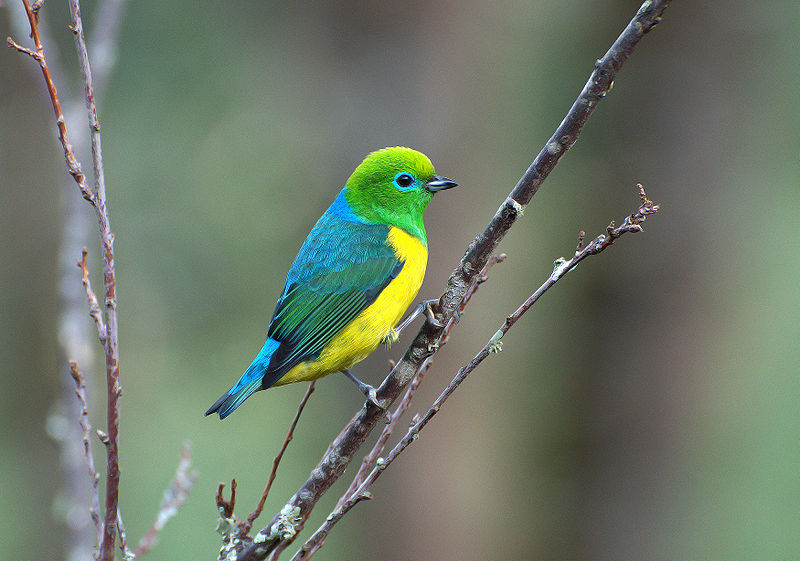
\includegraphics[scale=0.5]{figuras/abntex2-modelo-livro-bandeirinha.jpg}
\fonte{Autoria própria.}
\end{figure}

\begin{quadro}[!htb]
\IBGEtab{%
\caption{Um exemplo de inserção de quadros.}%
\label{exquadro}
}{%
\renewcommand{\arraystretch}{2}
\begin{tabular}{|c|c|c|c|c|c|c|c|c|c|c|c|}
\hline
Atividade & Jan & Fev & Mar & Abr & Mai & Jun & Jul & Ago & Set & Out & Nov \\
\hline
Nome da atividade 01 & X & X & X & X &  &  &  &  &  &  & \\
\hline 
Nome da atividade 02 &  &  &  &  & X & X & X & X & X &  & \\
\hline 
Nome da atividade 03 &  &  &  &  &  &  &  & X & X & X & \\
\hline
Nome da atividade 04 &  &  &  &  &  &  &  &  & X & X & X \\
\hline
Nome da atividade 05 &  &  &  &  &  &  &  &  &  & X & X \\
\hline
\end{tabular}%
}{%
\fonte{Autoria própria.}%
%\nota{Esta é uma nota, que diz que os dados são baseados na regressão linear.}%
%\nota[Anotações]{Uma anotação adicional, que pode ser seguida de várias outras.}%
}
\end{quadro}

\newpage
\begin{scriptsize}
\estiloCodigo
\begin{lstlisting}[caption={Um exemplo de inserção de códigos.}, label=excodigo, captionpos=t]
    em.getTransaction().begin();
        String sql = "select c from Cliente c where c.cpf = :doc ";
        TypedQuery<Cliente> clientes = em.createQuery(sql, Cliente.class);
        clientes.setParameter("doc", cpf);
        em.getTransaction().commit();
        if (!clientes.getResultList().isEmpty()) {
            cli = clientes.getSingleResult();
        } else {
                cli = null;
        }  
    }
\end{lstlisting}
\fonte{Autoria própria.}
\end{scriptsize}

Outra coisa que será bastante necessária, especialmente neste capítulo, é o uso das citações. Basicamente, há três possibilidades de citação: a citação direta curta, a citação direta longa e a citação indireta. Veja alguns exemplos simples:

Para a citação direta curta, coloque o texto de no máximo 3 linhas entre aspas e, no final da sentença, use o comando \cite[s.n]{abntex2-wiki-como-customizar}.

Para a citação indireta, antes de colocar a ideia do(a) autor(a) com suas palavras dentro do seu trabalho, use o comando \citeonline{abntex2-wiki-como-customizar}.

Para a citação direta longa, use o comando
\begin{citacao}
Texto de citação direta longa, seguido da fonte com a indicação da página de onde aquele trecho foi retirado. \cite[p. 2]{abntex2-wiki-como-customizar}
\end{citacao}



